\documentclass[12pt]{beamer}
\usepackage[spanish]{babel}
\usepackage[utf8]{inputenc}
\usepackage{xcolor}
\usepackage{listings}
\usepackage{palatino}
\usepackage{fancyvrb}
\usepackage{amsmath}
\usepackage{graphics}

\usecolortheme{crane}
\usefonttheme{serif}

\title{Archivos}
\author{
  Roberto Bonvallet \\
  \url{roberto.bonvallet@usm.cl} \\
  \url{http://progra.8o.cl}
}

\lstloadlanguages{fortran}
\lstset{language=fortran,basicstyle=\small,%
        morestring=[b]',stringstyle=\it,showstringspaces=false}
\fvset{formatcom=\small,frame=single,gobble=6,commandchars=\\\{\}}

\begin{document}
  \begin{frame}
    \maketitle
  \end{frame}

  \begin{frame}
    \frametitle{El computador}
    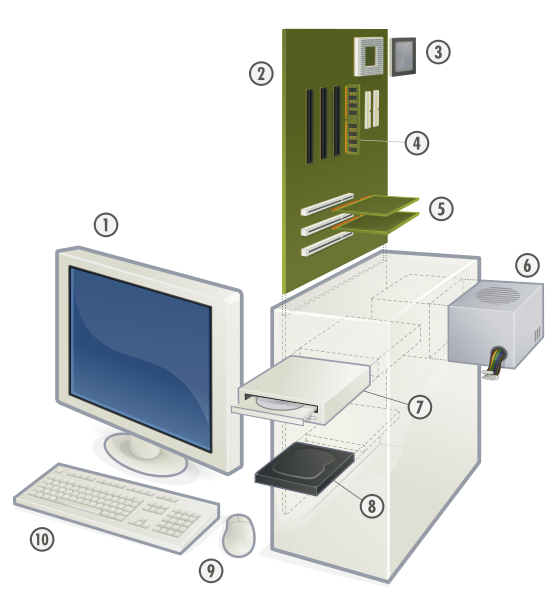
\includegraphics[scale=.4]{compu}
  \end{frame}

  \begin{frame}
    \frametitle{Unidades de almacenamiento}
    \begin{columns}[t]
      \column{0.5\textwidth}
        \begin{itemize}
          \item memoria RAM:
            \begin{itemize}
              \item volátil
              \item acceso directo
              \item rápida {\tiny($\sim$ns)}
              \item cara {\tiny(\$10k/GB)}
              \item poca capacidad {\tiny($\sim$GB)}
              \item contiene variables e instrucciones
            \end{itemize}
        \end{itemize}
      \column{0.5\textwidth}
        \begin{itemize}
          \item disco duro:
            \begin{itemize}
              \item persistente
              \item acceso secuencial
              \item lento {\tiny($\sim$ $\mu$s)}
              \item barato {\tiny(\$100/GB)}
              \item mucha capacidad {\tiny($\sim$TB)}
              \item contiene \alert{archivos}
            \end{itemize}
        \end{itemize}
    \end{columns}
  \end{frame}

  \begin{frame}[fragile]
    \frametitle{Archivos}
    \begin{itemize}
      \item \emph{Unit}: número asociado al archivo
      \item Operaciones:
        \begin{itemize}
          \item abrir un archivo
          \item escribir datos en el archivo
          \item leer datos del archivo
          \item guardar el archivo
        \end{itemize}
        \pause
        \begin{lstlisting}[frame=single,gobble=6]
          open (unit=10, file='archivo.txt', ...)
          write (10, *), a
          read (10, *), b
          close (10)
        \end{lstlisting}
        \pause
      \item Dos tipos de archivo:
        \begin{itemize}
          \item archivo de texto (``un string infinito'')
          \item archivo binario (``un arreglo infinito'')
        \end{itemize}

    \end{itemize}
    
\end{frame}

  %\begin{frame}
  %    \frametitle{Ver ejemplos}
  %\end{frame}

  %\begin{frame}
  %    \frametitle{Control 5}
  %    \pause

  %    Una canción tiene los siguientes datos: título, artista, álbum,
  %    duración (en segundos), fecha de grabación (día, mes y año).

  %    Escriba un programa que permita ingresar los datos de 100 canciones,
  %    y a continuación
  %    muestre los títulos de las canciones grabadas en abril. 

  %    Use registros llamados \texttt{fecha} y \texttt{cancion}.
  %\end{frame}

  \begin{frame}[fragile]
    \frametitle{Archivos de texto}
    \begin{itemize}
      \item Crear un archivo de texto (error si ya existe):
        \begin{lstlisting}[gobble=8,frame=single]
          open (unit=10, file='a.txt',           &
                action='write', status='new')
        \end{lstlisting}
      \item Crear un archivo de texto (sobreescribir si ya existe):
        \begin{lstlisting}[gobble=8,frame=single]
          open (unit=11, file='b.txt',           &
                action='write', status='old')
        \end{lstlisting}
      \item Abrir un archivo de texto para escribir al final de él:
        \begin{lstlisting}[gobble=8,frame=single]
          open (unit=12, file='c.txt',           &
                action='write', position='append')
        \end{lstlisting}
      \item Abrir un archivo de texto para leer de él:
        \begin{lstlisting}[gobble=8,frame=single]
          open (unit=13, file='d.txt', action='read')
        \end{lstlisting}
    \end{itemize}
    
\end{frame}

  \begin{frame}[fragile]
    \frametitle{Tipos de archivos}
    \begin{columns}
      \column{0.5\textwidth}
        Archivo de texto:\vspace{1ex}
        \begin{Verbatim}
          12478 91 -123
          32 54 192
          -277 10 90
          12 1 4
        \end{Verbatim}
      \column{0.5\textwidth}
        Archivo binario:\vspace{1ex}
        \begin{tabular}{|r|r|r|}\hline
          12478 & 91 & $-$123 \\\hline
             32 & 54 &    192 \\\hline
         $-$277 & 10 &     90 \\\hline
             12 & \phantom{0000}1 & \phantom{0000}4 \\\hline
        \end{tabular}
    \end{columns}
    \pause
    \begin{columns}
      \column{0.5\textwidth}
        \begin{lstlisting}[gobble=10]
          open(unit=10, &
               file='a.txt')

          read (10, *), x
          write (10, *), x
          close (10)
        \end{lstlisting}
      \column{0.5\textwidth}
        \begin{lstlisting}[gobble=10]
          open(unit=11,      &
               file='a.dat', &
               form='unformatted')
          read (11), x
          write (11), x
          close (11)
        \end{lstlisting}
    \end{columns}

\end{frame}

  \begin{frame}
    \frametitle{Ejercicio}
    Una asignatura tiene:
    año, semestre, código, nombre, número de alumnos.
    Escriba un programa
    que pida al usuario los datos de asignaturas
    y los agregue a un archivo binario \texttt{asignaturas.dat}.
  \end{frame}

  \begin{frame}
    \frametitle{Ejercicio}
    Escriba un programa que muestre los contenidos
    del programa \texttt{asignaturas.dat}.
  \end{frame}

  \begin{frame}
    \frametitle{Ejercicio}
    Escriba un programa que pida al usuario
    un año, un semestre y un código,
    y muestre el número de alumnos de esa asignatura.
  \end{frame}

  \begin{frame}
    \frametitle{Ejercicio}
    Escriba un programa que muestre los ramos del año 2010.
  \end{frame}

  \begin{frame}[fragile]
    \frametitle{Ejercicio}
    \small
    Los datos del archivo \texttt{alumnos.dat} tienen esta estructura:
    \begin{lstlisting}[basicstyle=\small,gobble=6]
      type :: alumno
          character(len=30) :: nombre, apellido
          character :: genero       ! 'M' o 'F'
          integer, dimension(3) :: notas
      end type alumno
    \end{lstlisting}
    Se desea enviar una carta a cada alumno con el mensaje:
    \begin{Verbatim}
      Estimad[o/a] alumn[o/a],
      usted ha [aprobado/reprobado]
      con promedio [p].
    \end{Verbatim}
    Escriba un programa que cree las cartas
    como archivos de texto llamados \texttt{carta-nombre-apellido.txt}.

\end{frame}

  \begin{frame}
    \frametitle{Ejercicio (continuación)}
    \small
    Escriba un programa que cree un reporte llamado \texttt{notas.txt}
    que tenga los apellidos y las notas
    de los alumnos del archivo \texttt{alumnos.dat}.

    Primero deben estar todos los alumnos aprobados,
    y a continuación los reprobados.
  \end{frame}

  \begin{frame}[fragile]
    \frametitle{Ejercicio (continuación)}
    \small
    Escriba un programa que cree un reporte llamado \texttt{estadisticas.txt}
    que tenga para cada alumno la siguiente información:
    \begin{Verbatim}
      Nombre completo: ...
      Nota más baja: ...
      Aprobado: [si/no]
      Sobre el promedio del curso: [si/no]
    \end{Verbatim}

\end{frame}

\end{document}
